%! suppress = Quote
%! suppress = TooLargeSection
% https://en.wikibooks.org/wiki/LaTeX/Colors
% Vertical allignment: https://tex.stackexchange.com/questions/9889/positioning-content-at-the-top-of-a-beamer-slide-by-default
%\documentclass[handout,aspectratio=43]{beamer}
%\documentclass[aspectratio=43]{beamer}
\documentclass[handout,aspectratio=169,usenames,dvipsnames]{beamer}
%\documentclass[aspectratio=169,usenames,dvipsnames]{beamer}

% https://www.overleaf.com/learn/latex/Questions/How_do_I_adjust_the_font_size%3F
\usepackage{moresize}

% https://tex.stackexchange.com/questions/231439/beamer-how-to-make-font-larger-for-page-numbers
\setbeamerfont{headline}{size=\ssmall}
\setbeamerfont{footline}{size=\ssmall}

\usepackage[utf8] {inputenc}
\usepackage[T2A] {fontenc}
\usepackage[english,russian] {babel}
\usepackage{indentfirst,verbatim}
\usepackage{listings,amsmath,amsfonts,amssymb,multicol}
\usepackage[makeroom]{cancel} %https://tex.stackexchange.com/questions/75525/how-to-write-crossed-out-math-in-latex
\usepackage{tabularx}
\usepackage{tikz}
\usepackage{proof}
\usepackage{soul} % https://tex.stackexchange.com/questions/23711/strikethrough-text
\usepackage{stmaryrd}
\usepackage{mathrsfs}
\usetikzlibrary{cd, babel}

% https://www.overleaf.com/learn/latex/Using_colours_in_LaTeX
\usepackage{xcolor}

\usetheme{CambridgeUS}
\usecolortheme{dolphin}

% https://9to5science.com/change-bullet-style-formatting-in-beamer
% https://tex.stackexchange.com/questions/185742/i-need-to-change-color-of-beamer-itemize-and-subitem-separately
%\setbeamertemplate{itemize items}[default]
%\setbeamertemplate{enumerate items}[default]
\setbeamertemplate{itemize item}{\scriptsize\raise1.25pt\hbox{\donotcoloroutermaths$\blacktriangleright$}}
\setbeamertemplate{itemize subitem}{\tiny\raise1.5pt\hbox{\donotcoloroutermaths$\blacktriangleright$}}
\setbeamertemplate{itemize subsubitem}{\tiny\raise1.5pt\hbox{\donotcoloroutermaths$\blacktriangleright$}}
\setbeamertemplate{enumerate item}{\insertenumlabel.}
\setbeamertemplate{enumerate subitem}{\insertenumlabel.\insertsubenumlabel}
\setbeamertemplate{enumerate subsubitem}{\insertenumlabel.\insertsubenumlabel.\insertsubsubenumlabel}

% https://tex.stackexchange.com/questions/642927/format-table-of-contents-in-beamer
\setbeamertemplate{section in toc}{%
    \leavevmode%
    % prevents the period to be printed with the first/last section option
    \ifnum\beamer@tempcount>\beamer@toclastsection
    \else
    \ifnum\beamer@tempcount>0
        {\color{blue}\inserttocsectionnumber.}
    \fi\fi%
    \inserttocsection\par%
}
\setbeamertemplate{subsection in toc}{%
    \leavevmode%
    % prevents the period to be printed with the first/last section option
    \ifnum\beamer@tempcount>0
        {\hspace{1em}\color{BlueViolet}\scriptsize\raise1.25pt\hbox{\donotcoloroutermaths$\blacktriangleright$}}
    \fi%
    \inserttocsubsection\par%
}

% Make font smaller
% https://tex.stackexchange.com/questions/56768/how-to-set-a-small-default-font-size-with-beamer
%\geometry{paperwidth=140mm,paperheight=105mm}
\geometry{paperwidth=168mm,paperheight=105mm}

% Mk mathbf work https://tex.stackexchange.com/questions/166434/problem-with-the-mathbf-command
\usepackage{cmbright}
%\fontencoding{OT1}\fontfamily{cmbr}\selectfont %to load ot1cmbr.fd
%\DeclareFontShape{OT1}{cmbr}{bx}{n}{% change bx definition
%<->cmbrbx10%
%}{}
%\normalfont % back to normalfont

\beamertemplatenavigationsymbolsempty

\newcommand{\backupbegin}{
    \newcounter{framenumbervorappendix}
    \setcounter{framenumbervorappendix}{\value{framenumber}}
}
\newcommand{\backupend}{
    \addtocounter{framenumbervorappendix}{-\value{framenumber}}
    \addtocounter{framenumber}{\value{framenumbervorappendix}}
}

\newcommand{\sectionplan}[1]{\section{#1}%
\frame[noframenumbering]{\tableofcontents[currentsection]}
}

\newcommand{\subsectionplan}[1]{\subsection{#1}%
\frame[noframenumbering]{\tableofcontents[currentsubsection]}
}

\newcommand{\haskellsn}[1]{\lstinline[language=Haskell]{#1}}

\newcommand{\sembr}[1]{\llbracket{#1}\rrbracket}

\newcommand{\funcExpr}[1]{\begingroup\color{blue}#1\endgroup}

\newcommand{\predicate}[1]{\begingroup\color{red}#1\endgroup}

\newcommand{\err}[0]{\textcolor{red}{ошибка}}

% https://tex.stackexchange.com/questions/116595/highlighting-haskell-listings-in-large-tex-document
\lstset{
    language=Haskell,
    basicstyle=\footnotesize,
    escapeinside={``}{``}
}

% Color code
% https://tex.stackexchange.com/questions/99475/how-to-invoke-latex-with-the-shell-escape-flag-in-texstudio-former-texmakerx
\usepackage{minted}
\setminted{xleftmargin=\parindent, autogobble, escapeinside=\#\#}
%\usemintedstyle{emacs}

% https://tex.stackexchange.com/questions/70448/dont-count-backup-slides
\usepackage{appendixnumberbeamer}
\usepackage{blkarray}
\usepackage{hyperref}
\usepackage{mathtools}
\usepackage{color}
\usepackage{graphicx}
\usepackage{wasysym}

% Speaker notes
% https://tex.stackexchange.com/questions/114219/add-notes-to-latex-beamer
% https://tex.stackexchange.com/questions/35444/split-beamer-notes-across-multiple-notes-pages/35496#35496
%--------------------------------------
%\setbeameroption{show notes on second screen=right} % enable speaker notes
%--------------------------------------

\author[Андрей Стоян]{Стоян Андрей Сергеевич \\ {\footnotesize научный руководитель: к.~ф.-м.~н.} Москвин Денис Николаевич \\ {\footnotesize научный консультант:} Новожилов Дмитрий Павлович}
\institute[ИТМО/SE]{Университет ИТМО\\Разработка программного обеспечения/Software engineering}

\title[Дизайн и разработка Self-типов для языка Kotlin]{Дизайн и разработка Self-типов для языка Kotlin}
\date{Санкт-Петербург 2023г.}

\begin{document}

    \maketitle

%    11 слайдов
%    4 - введение + цели и задачи
%    6 - основная часть
%       * 1 - анализ решений в других языках
%       * 3 - интеграция в типовую систему
%       * 1 - реализация в компиляторе
%       * 1 - тестирование реализации
%    1 - результаты


    \section{Введение}


    \subsection{Проблематика}

    \mode<all>
    \begin{frame}[fragile]{Рекурсивные дженерики}
        \note<1->{0:30 - 1:15}
        \note<1>{
            \begin{enumerate}
                \item Система типов языка Котлин недостаточно гибка на данный момент
                \item В качестве примера рассмотрим следующую задачу
                \item Метод add персистентной коллекции возвращает новую коллекцию с уже добавленным элементом
                \item Чтобы вернуть именно тот тип, на котором он был вызван, введём типовой параметр с рекурсивным ограничением
            \end{enumerate}
        }
        \note<2>{
            \begin{enumerate}
                \item Этот параметр требуется распространить по всей иерархии наследования
            \end{enumerate}
        }
        \note<3>{
            \begin{enumerate}
                \item Чтобы воспользоваться интерфейсом, требуется отдельный типовой параметр
                \item И тогда add возвращает тип с нужным ограничением: можно вызывать специфичные для списка методы
            \end{enumerate}
        }

        Требуется выразить в типе, что метод возвращает тот же тип, на котором вызывается.

        \begin{block}{Пример: персистентные коллекции с рекурсивными ограничениями}
            \begin{minted}[escapeinside=??]{kotlin}
                interface PCollection<out E, ?\framebox{out S : PCollection<E, S>}?> {
                    fun add(value: @UnsafeVariance E): ?\framebox{S}?
                } ?\pause?
                interface PList<out E, ?\framebox{out S : PList<E, S>}?> : PCollection<E, ?\framebox{S}?> {
                    fun listSpecific()
                } ?\pause?
                fun <T, ?\framebox{L}?> test(xs: ?\framebox{L}?, x: T) where ?\framebox{L : PList<T, L>}? {
                    xs.add(x) /* : ?\framebox{L}? */ .listSpecific() }
            \end{minted}
        \end{block}

        \pause

        \begin{block}{Недостатки}
            \begin{itemize}
                \item Возникающий паттерн рекурсивного ограничения распространяется по всему коду
                \item Требуется явное приведение типов: \mintinline[escapeinside=??]{kotlin}|this as S|
                \item Однажды зафиксированный типовой аргумент \texttt{S} не может быть уточнён в наследниках
            \end{itemize}
        \end{block}
    \end{frame}
    \mode*

    \mode<all>
    \begin{frame}[fragile]{Добавление abstract override методов}
        \note<1->{1:15 - 1:45}

        \note<1>{
            \begin{enumerate}
                \item В базовом интерфейсе add возвращает коллекцию
            \end{enumerate}
        }
        \note<2>{
            \begin{enumerate}
                \item В наследнике помещается abstract override метод с более специфичным возвращаемым типом
            \end{enumerate}
        }
        \note<3>{
            \begin{enumerate}
                \item Теперь add возвращает тип своего ресивера --- список
            \end{enumerate}
        }

        Можно добавить переопределяющие методы с более специфичным возвращаемым типом.

        \begin{block}{Пример: персистентные коллекции с abstract override}
            \begin{minted}[escapeinside=??]{kotlin}
                interface PCollection<out E> {
                    fun add(value: @UnsafeVariance E): ?\framebox{PCollection<E>}?
                } ?\pause?
                interface PList<out E> : PCollection<E> {
                    abstract override fun add(value: @UnsafeVariance E): ?\framebox{PList<E>}?
                    fun listSpecific()
                } ?\pause?
                fun <T> test(xs: PList<T>, x: T) { xs.add(x)/* : ?\framebox{PList<T>}? */.listSpecific() }
            \end{minted}
        \end{block}

        \pause

        \begin{block}{Недостатки}
            \begin{itemize}
                \item Много рутинного кода: переопределить каждый метод в каждом наследнике
                \item Нет контроля компилятора, что abstract override методы не были забыты
                \item Работает только для возвращаемого типа (типы параметров обязаны совпадать)
            \end{itemize}
        \end{block}
    \end{frame}
    \mode*


    \subsection{Существующие решения}

    \begin{frame}[fragile]{Self-типы}
        \note<1->{1:45 - 2:15}

        \note<1>{
            \begin{enumerate}
                \item У описанной проблемы существует каноническое решение --- Self-типы
            \end{enumerate}
        }

        \begin{itemize}
            \item Вводится специальный тип \texttt{Self} (или \texttt{ThisType} в литературе)
            \item \texttt{Self} ссылается на тип наследника, на котором вызывается метод (\emph{тип ресивера})
            \item \texttt{Self} --- тип специального параметра \mintinline{kotlin}|this| (\emph{объекта ресивера})
            \item Подход не имеет описанных ранее недостатков
        \end{itemize}

        \pause

        \begin{block}{Пример: персистентные коллекции с Self-типами}
            \begin{minted}[escapeinside=??]{kotlin}
                interface PCollection<out E> {
                    fun add(value: @UnsafeVariance E): ?\framebox{Self}?
                } ?\pause?
                interface PList<out E> : PCollection<E> {
                    fun listSpecific()
                } ?\pause?
                fun <T> test(xs: PList<T>, x: T) {
                    xs.add(x) /* : ?\framebox{PList<T>}? */ .listSpecific()
                }
            \end{minted}
        \end{block}
    \end{frame}


    \section{Цель и задачи}

    \begin{frame}[fragile]{Цель и задачи}
        \note<1->{2:15 - 2:45}

        \begin{block}{Цель}
            Реализовать поддержку Self-типов для языка Kotlin.
        \end{block}

        \begin{block}{Задачи}
            \begin{enumerate}
                \item Проанализировать существующие решения
                \item Интегрировать Self-типы в типовую систему языка Kotlin
                \item Реализовать поддержку Self-типов в компиляторе kotlinc
                \item Протестировать полученную реализацию
            \end{enumerate}
        \end{block}
    \end{frame}


    \section{Ход работы}


    \subsection{Анализ существующих решений}

    \begin{frame}[fragile]{Существующие реализации Self-типов}
        \note<1->{2:45 - 3:15}

        \note<1>{
            \begin{enumerate}
                \item Рассмотрим существующие реализации Self-типов в других языках
                \item В языках без наследования Self-типы присутствуют в виде рекурсивных типов
            \end{enumerate}
        }

        \begin{block}{Языки без наследования: Haskell, Rust...}
            Self-типы присутствуют в виде рекурсивных типов.
        \end{block}

        \pause
        \note<2>{
            \begin{enumerate}
                \item Для объектно-ориентированных языков ситуация сложнее
                \item Так как наследник с Self-типом не всегда является подтипом
                \item Из-за этого многие реализации небезопасны
                \item В Swift реализация безопасна, но существенно ограничена
            \end{enumerate}
        }

        \begin{block}{ООП языки, поддерживющие Self-типы}
            В системе с Self-типами наследник не всегда является подтипом~[\href{https://dl.acm.org/doi/pdf/10.1145/96709.96721}{Cook et al, 1989}].
            \begin{itemize}
                \item Python, TypeScript (this-типы), Java с плагином Manifold --- небезопасная реализация
                \item Swift --- безопасная, поддерживается исходящая позиция, остальные ограничены
            \end{itemize}
        \end{block}

        \pause
        \note<3>{
            \begin{enumerate}
                \item Существует современная работа, вводящая Self-типы в Java
                \item ....
                \item В дальнейшей работе я адаптирую проверенные безопасные решения к специфике языка Kotlin
                \item Для этого я определил во-первых правила подтипизации для Self-типа
            \end{enumerate}
        }

        \begin{block}{Формализм CoreThisJava \href{https://dl.acm.org/doi/pdf/10.1145/2888392}{[ThisType for Object-Oriented Languages, Rye et al, 2016]}}
            \begin{itemize}
                \item Пересмотрена подтипизация для поддержки Self-типов в контравариантной позиции
                \item Введены виртуальные конструкторы для создания новых значений Self-типа
                \item Формально доказана безопасность приведённой системы типов
            \end{itemize}
        \end{block}
    \end{frame}


    \subsection{Интеграция Self-типов в типовую систему Kotlin}

    \begin{frame}[fragile]{Правила подтипизации для Self-типа}
        \note<1->{3:15 - 4:00}

        \begin{block}{Граница Self-типа}
            Тип $B$ является границей Self-типа (обозначение \underline{$Self(B)$}), если $B$~--- наиболее общий тип ресивера, на котором этот метод может быть вызван.
            Совпадает с типом текущего класса.
        \end{block}

        \pause

        \begin{block}{Правила подтипизации для Self-типа}
            \begin{enumerate}
                \item \label{itm:covariant-bound} $B <: A \iff Self(B) <: Self(A)$ для возможности переопределения методов с \texttt{Self}
                \item \label{itm:this-subtype} $B <: A \iff Self(B) <: A$, чтобы код с \mintinline{kotlin}|this| оставался типизируемым
                \item \label{itm:any-nothing} $Nothing <: Self(A)$ и $Self(A) <: Any$
                \item \label{itm:no-subtypes} $B \bcancel{<:} Self(A)$, если $B$ не подходит под правила (\ref{itm:covariant-bound}) и (\ref{itm:any-nothing})
            \end{enumerate}
        \end{block}

        \pause

        \begin{block}{Безопасность присваиваний}
            \begin{enumerate}
                \item \mintinline{kotlin}|this|, ссылающийся на ресивер $C$, имеет тип $Self(C)$
                \item Правило (\ref{itm:no-subtypes}) не позволяет использовать посторонний объект в качестве $Self$
            \end{enumerate}
        \end{block}
    \end{frame}

    \begin{frame}[fragile]{Создание новых объектов Self-типа}
        \note<1->{4:00 - 4:30}

        \note<1>{
            \begin{enumerate}
                \item Для многих важных приложений, например, персистентных коллекций, необходимо уметь создавать новые объекты Self-типа
                \item Для этого необходимо, чтобы тип создаваемого объекта всегда был подтипом типа ресивера
            \end{enumerate}
        }

        Новый объект \mintinline{kotlin}|C(..)| имеет Self-тип $\iff$ \mintinline{kotlin}|C::class isSubtypeOf this.getClass()|\footnote{Условие должно выполняться всегда и быть проверяемо статически в месте создания объекта.}.

        \pause

        \begin{block}{Существующие решения}
            Ненаследуемые методы [\href{http://www.fos.kuis.kyoto-u.ac.jp/~igarashi/papers/pdf/thistype-SAC09.pdf}{Saito et al, 2009}] и виртуальные конструкторы [\href{https://www.researchgate.net/profile/Sukyoung-Ryu/publication/254004584_Exact_type_parameterization_and_ThisType_support/links/54b90ed10cf269d8cbf72d01/Exact-type-parameterization-and-ThisType-support.pdf}{Na et al, 2012}].
        \end{block}

        \begin{block}{Недостатки существующих решений}
            \begin{itemize}
                \item Вводятся специальные виды методов, не консистентных остальным
                \item Требуется много рутинного кода
            \end{itemize}
        \end{block}

        \pause

        \begin{block}{Правило новых значений Self-типа для Kotlin}
            \begin{itemize}
                \item Класс \texttt{C} должен быть финальным
                \item Тип \mintinline{kotlin}|this|\footnote{Ресивер текущей декларации (c типом границы Self-типа)} либо равен \texttt{С}, либо включает \texttt{C} после smart-cast
                \item Тип \texttt{C} объявлен в том же модуле, в котором создаётся объект\footnote{Иначе открытие класса нарушало бы совместимость исходных кодов}
            \end{itemize}
        \end{block}
    \end{frame}

    \begin{frame}{Позиции Self-типа}
        \note<1->{4:30 - 5:00}

        \note<1>{
            \begin{enumerate}
                \item Важнейшую роль в безопасности Self-типов выбор допустимых позиций
                \item ....
            \end{enumerate}
        }

        \begin{block}{Существующие решения}
            \begin{itemize}
                \item Только позиция возвращаемого типа (как в Swift)
                \begin{itemize}
                    \item Отсекаются полезные сценарии использования (например, рекурсивные структуры данных)
                \end{itemize}
                \item Контравариантные позиции [\href{https://dl.acm.org/doi/pdf/10.1145/96709.96721}{Inheritance is not subtyping, Cook et al, 1989}]
                \begin{itemize}
                    \item Требуются массивные изменения в системе типов
                    \begin{itemize}
                        \item Отношение matching'а вместо подтипизации [\href{https://www.researchgate.net/profile/Kim-Bruce-2/publication/221496196_Subtyping_Is_Not_a_Good_Match_for_Object-Oriented_Languages/links/09e415122545c6d7a4000000/Subtyping-Is-Not-a-Good-Match-for-Object-Oriented-Languages.pdf}{Bruce et al, 1996}]
                        \item Разделение точных и экзистенциальных типов, локальное уточнение [\href{https://citeseerx.ist.psu.edu/document?repid=rep1&type=pdf&doi=a9d601d3bf8c921748902d58078d0a1b28f6ec4d}{Saito et al, 2009}]
                        \item Именованные wildcard'ы и точные типовые параметры [\href{https://www.researchgate.net/profile/Sukyoung-Ryu/publication/254004584_Exact_type_parameterization_and_ThisType_support/links/54b90ed10cf269d8cbf72d01/Exact-type-parameterization-and-ThisType-support.pdf}{Na et al, 2012}]
                    \end{itemize}
                    \item Случаи использования реализуются через контекстные ресиверы языка Kotlin
                \end{itemize}
            \end{itemize}
        \end{block}

        \pause
        \note<2>{
            \begin{enumerate}
                \item Поэтому было решено ограничить использование Self-типов на ковариантные позиции
                \item Таким образом, были описаны правила типизации для Self-типов
                \item Далее с их помощью, я реализовал поддержку Self-типов к компиляторе Kotlin
            \end{enumerate}
        }

        \begin{block}{Правило позиций Self-типа для Kotlin}
            Разрешается использовать Self-тип только в ковариантных позициях.
        \end{block}
    \end{frame}


    \subsection{Реализация Self-типов в компиляторе kotlinc}

    \begin{frame}{Реализация Self-типов в компилиторе Kotlin}
        \note<1->{5:00 - 5:30}

        \begin{enumerate}
            \item Идентификатор \texttt{Self} введён как ключевое слово языка
            \item Введён новый вид типов --- Self-типы
            \item Правила системы типов Kotlin дополнены для работы с Self-типами:
            \begin{itemize}
                \item Правило подтипизации
                \item Правило определения непосредственных супертипов
                \item Правило вычисления ближайших общих супертипов
            \end{itemize}
            \item Реализован типовой скоуп\footnote{Типовой скоуп --- сервис компилятора, возвращающий множество функций, для которых объект данного типа может быть использован как ресивер: $(plus : String\ldotp(String) \to String) \in scope(String)$.}, подставляющий тип ресивера вместо Self-типа
            \item Реализовано преобразование, подменяющее Self-тип на его границу и метаинформацию, при переходе к промежуточному представлению бекенда компилятора (IR)
        \end{enumerate}
    \end{frame}


    \subsection{Тестирование реализации}

    \begin{frame}{Тестирование реализации}
        \note<1->{5:30 - 6:00}

        \begin{itemize}
            \item Протестирована компилируемость различных сценариев использования
            \begin{itemize}
                \item Self-типы в различных позициях
                \item Создание новых объектов Self-типа
            \end{itemize}
            \item Протестирован недопуск системой типов некорректных программ с Self-типами:
            \begin{itemize}
                \item Использующих ссылку на другой объект, где ожидается Self-тип
                \item Некорректно создающих новый объект, где ожидается Self-тип
                \item Использующих Self-тип в небезопасной позиции
            \end{itemize}
            \item Протестирована работоспособность кода с Self-типами
        \end{itemize}
    \end{frame}


    \section{Результаты}

    \begin{frame}{Результаты}
        \note<1->{6:00 - 6:30}

        \begin{enumerate}
            \item Проанализированы существующие реализации Self-типов в других языках на предмет мер по обеспечению безопасности системы с Self-типами
            \item Self-типы интегрированы\footnote{\url{https://github.com/winter-yuki/kotlin-self-types}} в типовую систему языка Kotlin путём доопределения правил типизации с опорой на существующие решения
            \item Поддержка Self-типов реализована\footnote{\url{https://github.com/winter-yuki/kotlin/tree/self-types}} в компиляторе kotlinc за счет добавления специального вида типов и скоупа подстановки Self-типов
            \item Полученная реализация протестирована на предмет допуска кода валидных сценариев использования и отвержения небезопасного кода
        \end{enumerate}
    \end{frame}


    \appendix


    \section{Дополнительные слайды}


    \subsection{Материалы}

    \begin{frame}{Материалы}
        %! suppress = LineBreak
        \begin{enumerate}
            \item \href{https://youtrack.jetbrains.com/issue/KT-6494}{\color{blue} YouTrack: Запрос на добавление Self-типов в Kotlin}
            \item Cook, William R., Walter Hill, and Peter S. Canning. 1989. <<Inheritance is not subtyping>>. Proceedings of the 17th ACM SIGPLAN-SIGACT symposium on Principles of programming languages. {\color{blue}\url{https://cs.rice.edu/~javaplt/papers/Inheritance.pdf}}
            \item Sukyoung Ryu. 2016. <<ThisType for Object-Oriented Languages: From Theory to Practice>>. ACM Trans. Program. Lang. Syst. 38, 3, Article 8 (May 2016), 66 pages. {\color{blue}\url{https://dl.acm.org/doi/10.1145/2888392}}
            \item \href{https://github.com/manifold-systems/manifold/blob/master/manifold-deps-parent/manifold-ext/README.md\#the-self-type-with-self}{\color{blue} Self-типы как плагин для Java}
            \item \href{https://docs.swift.org/swift-book/documentation/the-swift-programming-language/types/\#Self-Type}{\color{blue} Swift: Self-типы}
            \item \href{https://peps.python.org/pep-0673/}{\color{blue} Python: Self-типы PEP}
            \item \href{https://www.typescriptlang.org/docs/handbook/2/classes.html\#this-types}{\color{blue}TypeScript: this-типы}
        \end{enumerate}
    \end{frame}


    \subsection{Kotlin}

    \begin{frame}{Вариантность}
        \begin{block}{Вариантность типового параметра}
            \begin{itemize}
                \item Определят, в каких позициях можно использовать этот типовой параметр
                \item Задаёт отношение подтипизации между параметризованными типами
            \end{itemize}
        \end{block}
        \begin{block}{Инвариантные типовые параметры: \mintinline[escapeinside=??]{kotlin}|interface Inv<T> { fun id(x: ?\framebox{T}?): ?\framebox{T}? }|}
            \begin{itemize}
                \item Можно использовать в произвольных позициях в декларациях методов
                \item Не устанавливает отношения подтипизации: \texttt{Inv<B> !<:> Inv<A>}
            \end{itemize}
        \end{block}
        \begin{block}{Ковариантные типовые параметры: \mintinline[escapeinside=??]{kotlin}|interface Out<?\framebox{out}? T> { fun produce(): ?\framebox{T}? }|}
            \begin{itemize}
                \item Можно использовать в исходящих позициях в декларациях методов
                \item Устанавливает прямое отношение подтипизации: \texttt{B <: A => Out<B> <: Out<A>}
            \end{itemize}
        \end{block}
        \begin{block}{Контравариантные типовые параметры: \mintinline[escapeinside=??]{kotlin}|interface In<?\framebox{in}? T> { fun accept(x: ?\framebox{T}?) }|}
            \begin{itemize}
                \item Можно использовать во входящих позициях в декларациях методов
                \item Устанавливает обратное отношение подтипизации: \texttt{B <: A => In<B> :> In<A>}
            \end{itemize}
        \end{block}
    \end{frame}


    \subsection{Мотивация: сценарии использования}

    \begin{frame}[fragile]{Рекурсивные структуры данных}
        Также Self-типы помогают строить рекурсивные структуры данных из вершин одного типа:
        \begin{minted}[escapeinside=??]{kotlin}
            // исходящая контравариантная позиция
            abstract class Node<out T>(val value: T, val children: List<?\framebox{Self}?>)
            class BetterNode<out T>(value: T, children: List<?\framebox{Self}?> = emptyList()) :
                Node<T>(value, children) {
                fun betterSpecific() = println(value)
            }

            fun test() {
                val betterTree = BetterNode(value = 2, children =
                    listOf<?\framebox{BetterNode<Int>}?>(
                        BetterNode(1, listOf(BetterNode(0))),
                        BetterNode(4, listOf(BetterNode(3), BetterNode(5)))))
                betterTree.children
                    .flatMap { it.children }
                    .forEach { it.betterSpecific() } // Печатает "0 3 5"
            }
        \end{minted}
    \end{frame}

    \begin{frame}[fragile]{Шаблон <<Абстрактная фабрика>>}
        Пусть требуется по элементу типизируемым образом получить породившую его фабрику.

        \begin{minted}[escapeinside=??]{kotlin}
            abstract class Element<out F : Factory>(val factory: F)

            interface Factory {
                fun create(): Element<?\framebox{Self}?> // ковариантная исходящая позиция
            }

            abstract class SpecificFactory : Factory {
                abstract fun doSpecific()
            }

            fun <F : SpecificFactory> test(element: Element<F>) {
                entity.factory.doSpecific()
            }
        \end{minted}
    \end{frame}

    \begin{frame}[fragile]{Шаблон <<Наблюдатель>>}
        \begin{columns}
            \begin{column}{0.48\textwidth}
                Абстрагируем логику регистрации и нотификации наблюдателей:
                \begin{minted}[escapeinside=??]{kotlin}
                    abstract class AbstractObservable {
                        private val observers =
                            mutableListOf<(Self) -> Unit>()

                        // контравариантная входная позиция
                        fun observe(
                            observer: (?\framebox{Self}?) -> Unit
                        ) {
                            observers += observer
                        }
                        private fun notifyObservers() {
                            observers.forEach { observer ->
                                observer(?\framebox{this}?)
                            }
                        }
                    }
                \end{minted}
            \end{column}

            \begin{column}{0.49\textwidth}
                \vspace{-0.5em}
                \begin{minted}[escapeinside=??]{kotlin}
                    class Entity : AbstractObservable {
                        var color: Color = Color.Purple
                            set(new: Color) {
                                field = new
                                notifyObservers()
                            }
                    }

                    fun observer(entity: ?\framebox{Entity}?) {
                        println("New: ${it.color}")
                    }

                    fun test() {
                        val entity = Entity()
                        entity.observe(::observer)
                        // Печатает "New: Color.Blue"
                        entity.color = Color.Blue
                    }
                \end{minted}
            \end{column}
        \end{columns}
    \end{frame}

    \begin{frame}[fragile]{Алгебры}
        Наследник не подтип, если рекурсивный тип стоит в контравариантной позиции\footnote{\href{https://dl.acm.org/doi/pdf/10.1145/96709.96721}{[Inheritance is not subtyping, Cook et al, 1989]}}.
        \begin{minted}{kotlin}
            interface Semigroup {
                infix fun add(other: Self): Self
            }
        \end{minted}
        От использования рекурсивного типа можно отказаться с помощью контекстных ресиверов:
        \begin{minted}{kotlin}
            interface Semigroup<S> {
                infix fun S.add(other: S): S
            }
            interface Monoid<M> : Semigroup<M> {
                val empty: M
            }
            context(Monoid<T>)
            fun <T> concat(vararg xs: T): T =
                xs.fold(empty) { acc, x -> acc add a }
        \end{minted}
    \end{frame}


    \subsection{Решения в других языках}

    \begin{frame}[fragile]{Ассоциированные типы (abstract type members)}
        \begin{columns}[onlytextwidth]
            \begin{column}[t]{0.40\textwidth}
                \begin{itemize}
                    \item Поддерживаются в Scala и Swift
                    \item Аналогично рекурсивным дженерикам, но без зашумления клиентского кода
                    \item Сложны в реализации: отслеживание по какому пути получен ассоциированный тип
                    \item Запроса от пользователей на поддержку ассоциированных типов в Kotlin нет
                \end{itemize}
            \end{column}\hfill%
            \begin{column}[t]{0.58\textwidth}
                \begin{minted}[escapeinside=\#\#]{scala}
                    trait PCollection[T] {
                      #\framebox{type S}#
                      def add(x: T): #\framebox{S}#
                    }

                    trait PList[T] extends PCollection[T] {
                      #\framebox{type S <: PList[T]}#
                      def listSpecific: Unit
                    }

                    class PListImpl[T] extends PList[T] {
                      #\framebox{type S = PListImpl[T]}#
                      override def add(x: T): #\framebox{PListImpl[T]}# = // ..
                      override def listSpecific: Unit = // ...
                    }
                \end{minted}
            \end{column}
        \end{columns}
    \end{frame}

    \begin{frame}[fragile]{TypeScript: небезопасность системы типов}
        \begin{minted}{typescript}
            class Box {
              sameAs(other: this): boolean { /* ... */ }
            }
            class DerivedBox extends Box {
              otherContent: string = "?";
              sameAs(other: this): boolean {
                if (other.otherContent === undefined) {
                  console.log("broken")
                }
                /* ... */
              }
            }
            const base = new Box();
            const derived = new DerivedBox();
            function test(x: Box): boolean { return x.sameAs(base) }
            test(derived) // Печатает "broken"
        \end{minted}
    \end{frame}

    \begin{frame}{Swift}
        \begin{itemize}
            \item Существует полная поддержка \href{https://docs.swift.org/swift-book/documentation/the-swift-programming-language/types/\#Self-Type}{\color{blue}Self-типов} для простой исходящей позиции
            \item Для методов классов Self-тип доступен только для исходящей позиции
            \item Если декларация метода протокола\footnote{Протоколы --- механизм специального полиморфизма как трейты или классы типов} содержит \href{https://docs.swift.org/swift-book/documentation/the-swift-programming-language/generics/\#Associated-Types}{\color{blue}ассоциированный тип} или Self-тип не в простой исходящей позиции:
            \begin{itemize}
                \item Запрещено вызывать такие методы виртуально на \mintinline{swift}|any Protocol|
                \item Можно вызывать, если протокол является ограничением типового параметра или при мономорфизации на \mintinline{swift}|some Protocol|
                \item Реализующий класс обязан заменить такие вхождения Self-типа на себя
                \item Ситуация становится аналогична языкам без наследования
            \end{itemize}
            \item Ассоциированные типы так же позволяют эмулировать Self-типы, но на один уровень иерархии и с дополнительными приведениями типа
            \item Self-типы в расширениях ссылаются на расширяемый тип
        \end{itemize}
    \end{frame}


    \subsection{Формализация}

    \begin{frame}[fragile]{Формализация Self-типов --- рекурсивные типы}
        \note<1->{3:00 - 3:30}

        Тип объекта формализуется в расширенном $\lambda$-исчислении через тип записи.
        \begin{block}{Правило подтипизации для типов записей}
            \[
                %! suppress = EscapeAmpersand
                \infer{
                    \{x_1 : \sigma_1, \ldots, x_k : \sigma_k, \ldots, x_n : \sigma_n\}
                    <:
                    \{x_1 : \tau_1, \ldots, x_k : \tau_n\}
                }{\sigma_1 <: \tau_1 & \ldots & \sigma_k <: \tau_k}
            \]
        \end{block}

        \vspace{-1em}
        \begin{columns}[onlytextwidth]
            \begin{column}[t]{0.485\textwidth}
                \begin{block}{Пример: тип объекта одномерной точки}
                    \vspace{-1.2em}
                    \begin{align*}
                        T &= \{ x : int, equal : T \to bool \} \\
                        T &= \mu t \ldotp \{ x : int, equal : t \to bool \}
                    \end{align*}
                \end{block}
            \end{column}\hfill%
            \begin{column}[t]{0.485\textwidth}
                \begin{block}{Правило подтипизации рекурсивных типов}
                    \begin{equation*}
                        \infer[\text{Amber rule}]{
                            \Gamma \vdash \mu s\ldotp \sigma[s] <: \mu t\ldotp \tau[t]
                        }{
                            \Gamma, s <: t \vdash \sigma[s] <: \tau[t]
                        }
                    \end{equation*}
                \end{block}
            \end{column}
        \end{columns}

        \begin{block}{Наследник не является подтипом [Inheritance is not subtyping, Cook at al, 1989]}
            \vspace{-1em}
            \begin{align*}
                T &= \mu t \ldotp \{ x : int, equal : t \to bool \} \\
                T' &= \mu t \ldotp \{ x : int, equal : t \to bool, dist : int \}
            \end{align*}

            Рекурсивный тип входит в тип $equal$ в контравариантной позиции, значит, $T'$ не подтип $T$.
        \end{block}
    \end{frame}

    \begin{frame}{Традиционная подтипизация [\href{https://dl.acm.org/doi/pdf/10.1145/2888392}{Ryu et al, 2016}]}
        \begin{center}
            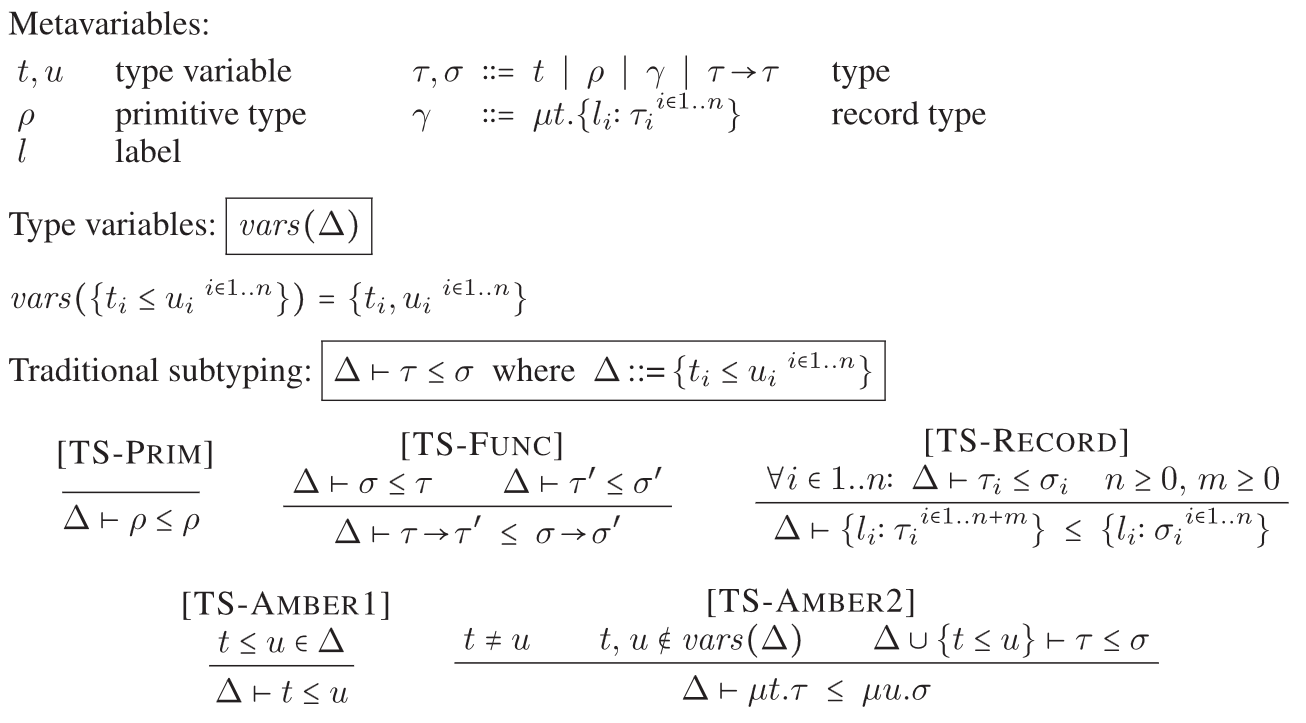
\includegraphics[height=0.85\textheight]{fig/subtyping1}
        \end{center}
    \end{frame}

    \begin{frame}{Пересмотренная подтипизация [\href{https://dl.acm.org/doi/pdf/10.1145/2888392}{Ryu et al, 2016}]}
        \begin{center}
            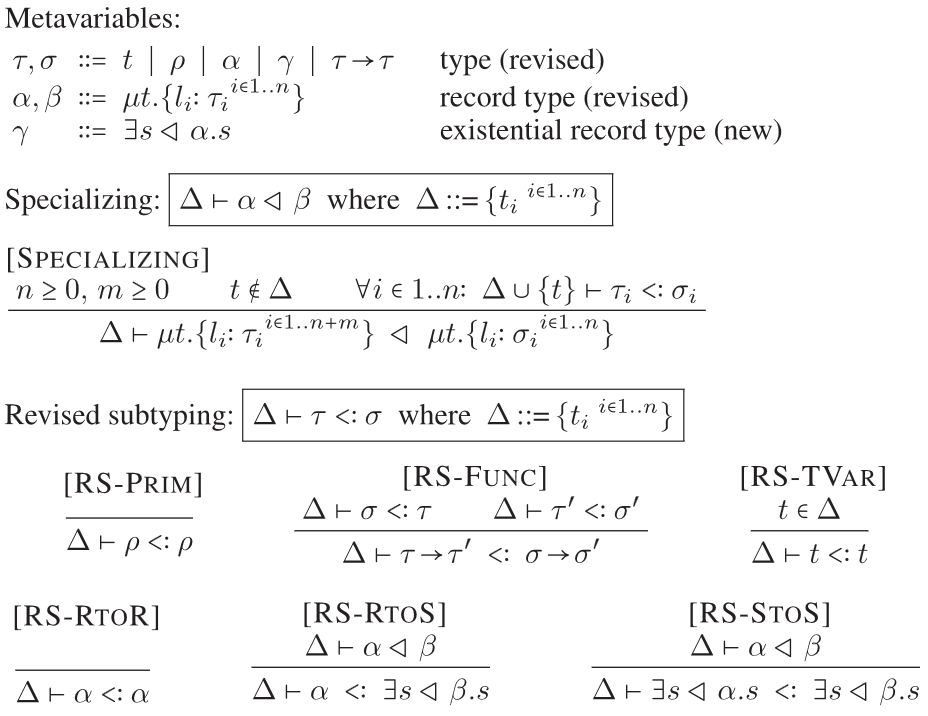
\includegraphics[height=0.85\textheight]{fig/subtyping2}
        \end{center}
    \end{frame}

    \begin{frame}{Соответствие правил для Kotlin с [\href{https://dl.acm.org/doi/pdf/10.1145/2888392}{Ryu et al, 2016}]}
        \begin{itemize}
            \item Self-тип --- это точный тип  $\mu t\ldotp \{ \overline{l_i : \tau_i} \}$ (exact type)
            \item А любой другой --- экзистенциальный тип $\exists s \triangleleft \alpha \ldotp s$ (inexact type)
        \end{itemize}

        \begin{block}{Подтипизация}
            Точный тип может быть подтипом экзистенциального, но не наоборот:
            \begin{columns}[onlytextwidth]
                \begin{column}[t]{0.485\textwidth}
                    \[
                        \infer[\text{RS-RtoS}]{
                            \Delta \vdash \alpha <: \exists s \triangleleft \beta \ldotp s
                        }{
                            \Delta \vdash \alpha \triangleleft \beta
                        }
                    \]
                \end{column}\hfill%
                \begin{column}[t]{0.485\textwidth}
                    \[
                        \infer[\text{Self-NoSelf}]{
                            \Delta \vdash Self(A) <: B
                        }{
                            \Delta \vdash A <: B
                        }
                    \]
                \end{column}
            \end{columns}
        \end{block}

        \begin{block}{Материализация}
            Материализация сходна с одним шагом развёртки изорекурсивного типа:
            \vspace{-1em}
            \begin{columns}[onlytextwidth]
                \begin{column}[t]{0.41\textwidth}
                    \[
                        %! suppress = EscapeAmpersand
                        \infer[\text{Unfold-Self}]{
                            \Delta \vdash unfold(o) : [t \mapsto U]T
                        }{
                            U = \mu t \ldotp T & \Delta \vdash o : U
                        }
                    \]
                \end{column}\hfill%
                \begin{column}[t]{0.58\textwidth}
                    \[
                        %! suppress = EscapeAmpersand
                        \infer[\text{Unfold-NoSelf}]{
                            \Delta \vdash unfold(o) : [t \mapsto U']T
                        }{
                            U = \mu t \ldotp T
                            &
                            U' = \exists s \triangleleft U \ldotp s
                            &
                            \Delta \vdash o : U'
                        }
                    \]
                \end{column}
            \end{columns}
        \end{block}
    \end{frame}


    \subsection{Интеграция в типовую систему Kotlin}

    \begin{frame}[fragile]{Правило материализации}
        \begin{block}{Правило материализации}
            Self-тип в сигнатуре вызываемого метода всегда переписывается в тип ресивера.
        \end{block}
        \begin{block}{Безопасность Self-типов}
            \begin{enumerate}
                \item Значение Self-типа безопасно относительно материализации (правила выше)
                \item Если ресивер имеет тип $A \neq Self$, \texttt{Self} материализуется в $A$, а $A \bcancel{<:} Self(A)$
                \item Если ресивер имеет тип \texttt{Self(B)}, то \texttt{Self(A)} декларации материализуется в \texttt{Self(B)}, и известно, что значение ресивера безопасно, материализуемое значение безопасно
            \end{enumerate}
            % exit code 1
            \begin{minted}[escapeinside=??]{kotlin}
                abstract class A {
                    fun self(): Self = this
                    fun unsafeSelf(a: A): Self/*(A)*/ =
                        a    /* : A       */ .self() // : ?\colorbox{yellow}{A}?, ?\textcolor{red}{ошибка компиляции}?
                    fun safeSelf():       Self/*(A)*/ =
                        this /* : Self(A) */ .self() // : ?\colorbox{yellow}{Self(A)}?, ?\textcolor{junglegreen}{ok}?, Self(A) <: Self(A)
                }
            \end{minted}
        \end{block}
    \end{frame}

    \begin{frame}[fragile]{Некорректные присваивания}
        \begin{columns}[onlytextwidth]
            \begin{column}{0.99\textwidth}
                Если позволить типизировать как Self отличный от ресивера объект (не \mintinline{kotlin}|this|), дальнейшая материализация Self-типа может приводить к небезопасности системы типов:

                \begin{minted}[escapeinside=??]{kotlin}
                    abstract class A {
                        fun unsafeObj(a: A): Self = ?\textcolor{red}{a}?
                    }

                    class B : A() {
                        fun bOnly() {}
                    }

                    fun test(a: A, b: B) {
                        b.unsageObj(a) /* скоуп типа B */ .bOnly() // ?\err?, нет bOnly в A
                    }
                \end{minted}
            \end{column}\hfill%
            \begin{column}{0.0\textwidth}
            \end{column}
        \end{columns}
    \end{frame}

    \begin{frame}[fragile]{Некорректное создание новых объектов}
        \begin{columns}[onlytextwidth]
            \begin{column}[t]{0.46\textwidth}
                \vspace{0.5em}

                Для реализации персистентных и иммутабельных структур данных нужно иметь возможность создавать новый объект Self-типа.

                \vspace{1em}
                \begin{block}{В общем случае небезопасно}
                    \begin{itemize}
                        \item Создавать объект открытого класса
                        \item Создавать объект другого класса
                    \end{itemize}
                \end{block}
            \end{column}\hfill%
            \begin{column}[t]{0.50\textwidth}
                \begin{minted}[escapeinside=??]{kotlin}
                    open class A {
                        fun newOfOpenA(): Self = A()
                        fun newOtherQ(): Self = Q()
                    }

                    class Q : A() { fun qOnly() {} }
                    class P : A() { fun pOnly() {} }

                    fun test(q: Q, p: P) {
                        q.newOfOpenA() // скоуп типа Q для A
                         .qOnly()      // ?\err?
                        p.newOther()   // скоуп типа P для Q
                         .pOnly()      // ?\err?
                    }
                \end{minted}
            \end{column}
        \end{columns}
    \end{frame}

    \begin{frame}[fragile]{Безопасное создание новых объектов типа \texttt{Self(C)}}
        \begin{columns}[onlytextwidth]
            \begin{column}[t]{0.46\textwidth}
                \begin{block}{Ограничения}
                    \begin{itemize}
                        \item Класс \texttt{C} должен быть финальным
                        \item Тип \mintinline{kotlin}|this|\footnote{Ресивер текущей декларации (c типом bound'а Self-типа)} либо равен \texttt{С}, либо включает \texttt{C} после smart-cast
                        \item Тип \texttt{C} объявлен в том же модуле, в котором создаётся объект\footnote{Иначе открытие класса нарушало совместимость исходных кодов}
                    \end{itemize}
                \end{block}
            \end{column}\hfill%
            \begin{column}[t]{0.50\textwidth}
                \begin{minted}[escapeinside=??]{kotlin}
                    sealed interface Data {
                        data class One(var a: Int) : Data

                        data class Two(
                            var a: Int, var b: Int
                        ) : Data

                        fun copy(): Self = when (this) {
                            is One -> ?\colorbox{green}{One(a)}?   //: Self(One)
                            is Two -> ?\colorbox{green}{Two(a, b)}?//: Self(Two)
                        } // : Self(Data)
                    }
                \end{minted}
            \end{column}
        \end{columns}
    \end{frame}


    \subsection{Реализация Self-типов в компиляторе}

    \begin{frame}{Архитектура компилятора Kotlin (K2)}
        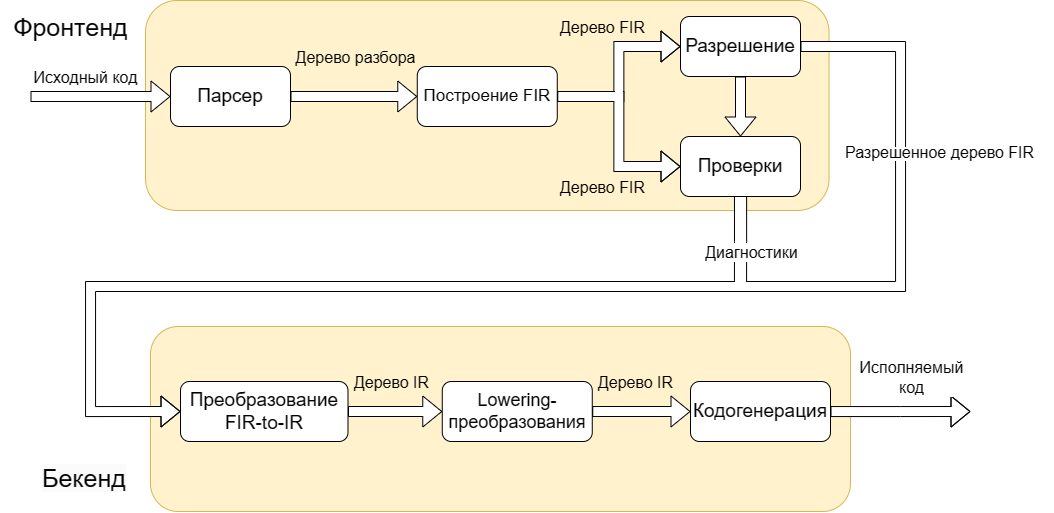
\includegraphics[width=\textwidth]{fig/arch}
    \end{frame}

\end{document}
